\documentclass{article}
\usepackage{graphicx} %package to manage images
\usepackage[utf8]{inputenc}
\usepackage[a4paper, total={6in, 8in}]{geometry}
\usepackage{xurl}
\usepackage{hyperref}
\usepackage{float}
\title{Relatório 7 \\ ROC curves}
\author{Pedro A. S. O. Neto}
\date{Agosto, 2023}

\begin{document}

\maketitle

\section{ROC curves}

\subsection{Propotions}

\begin{figure}[H]
  \caption{Mean proportion spent looking at particular AOIs}
  \noindent\makebox[\textwidth]{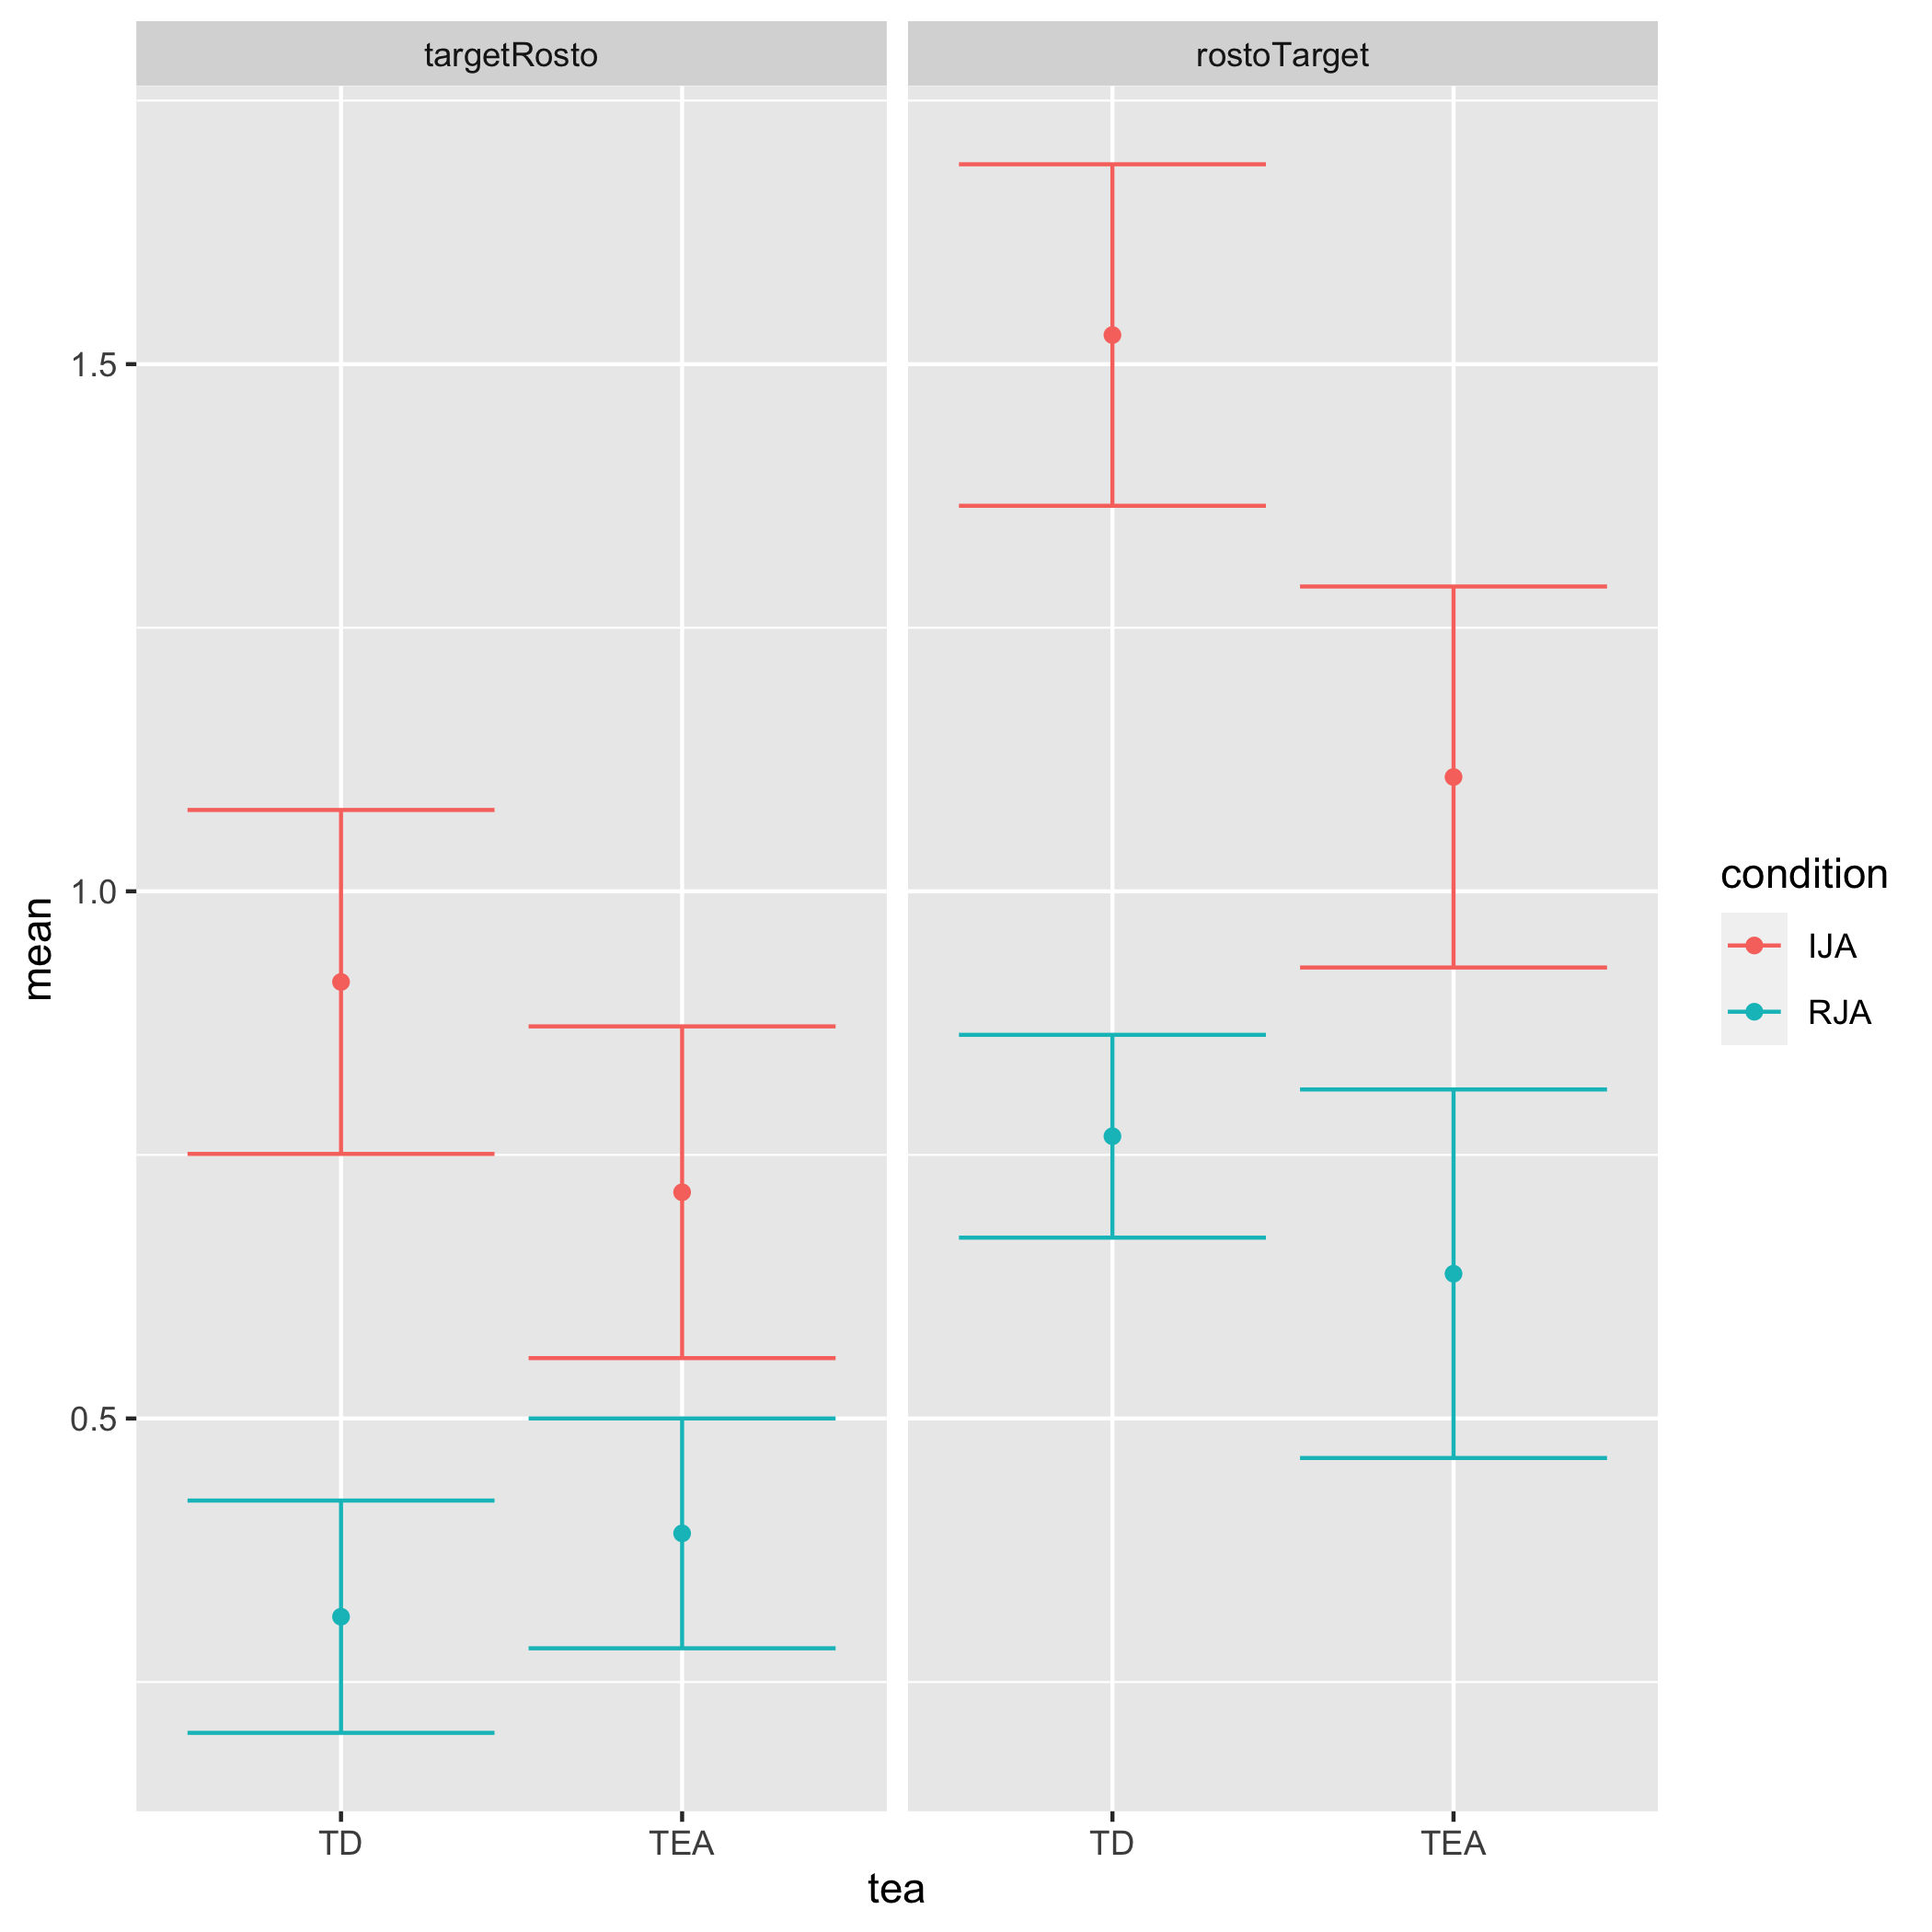
\includegraphics[scale=0.2]{./conditionVariableTEAProportion.png}}
  \centering
\end{figure}

\begin{figure}[H]
  \caption{ROC curves para fundoProportion em samples matched e não matched}
  \noindent\makebox[\textwidth]{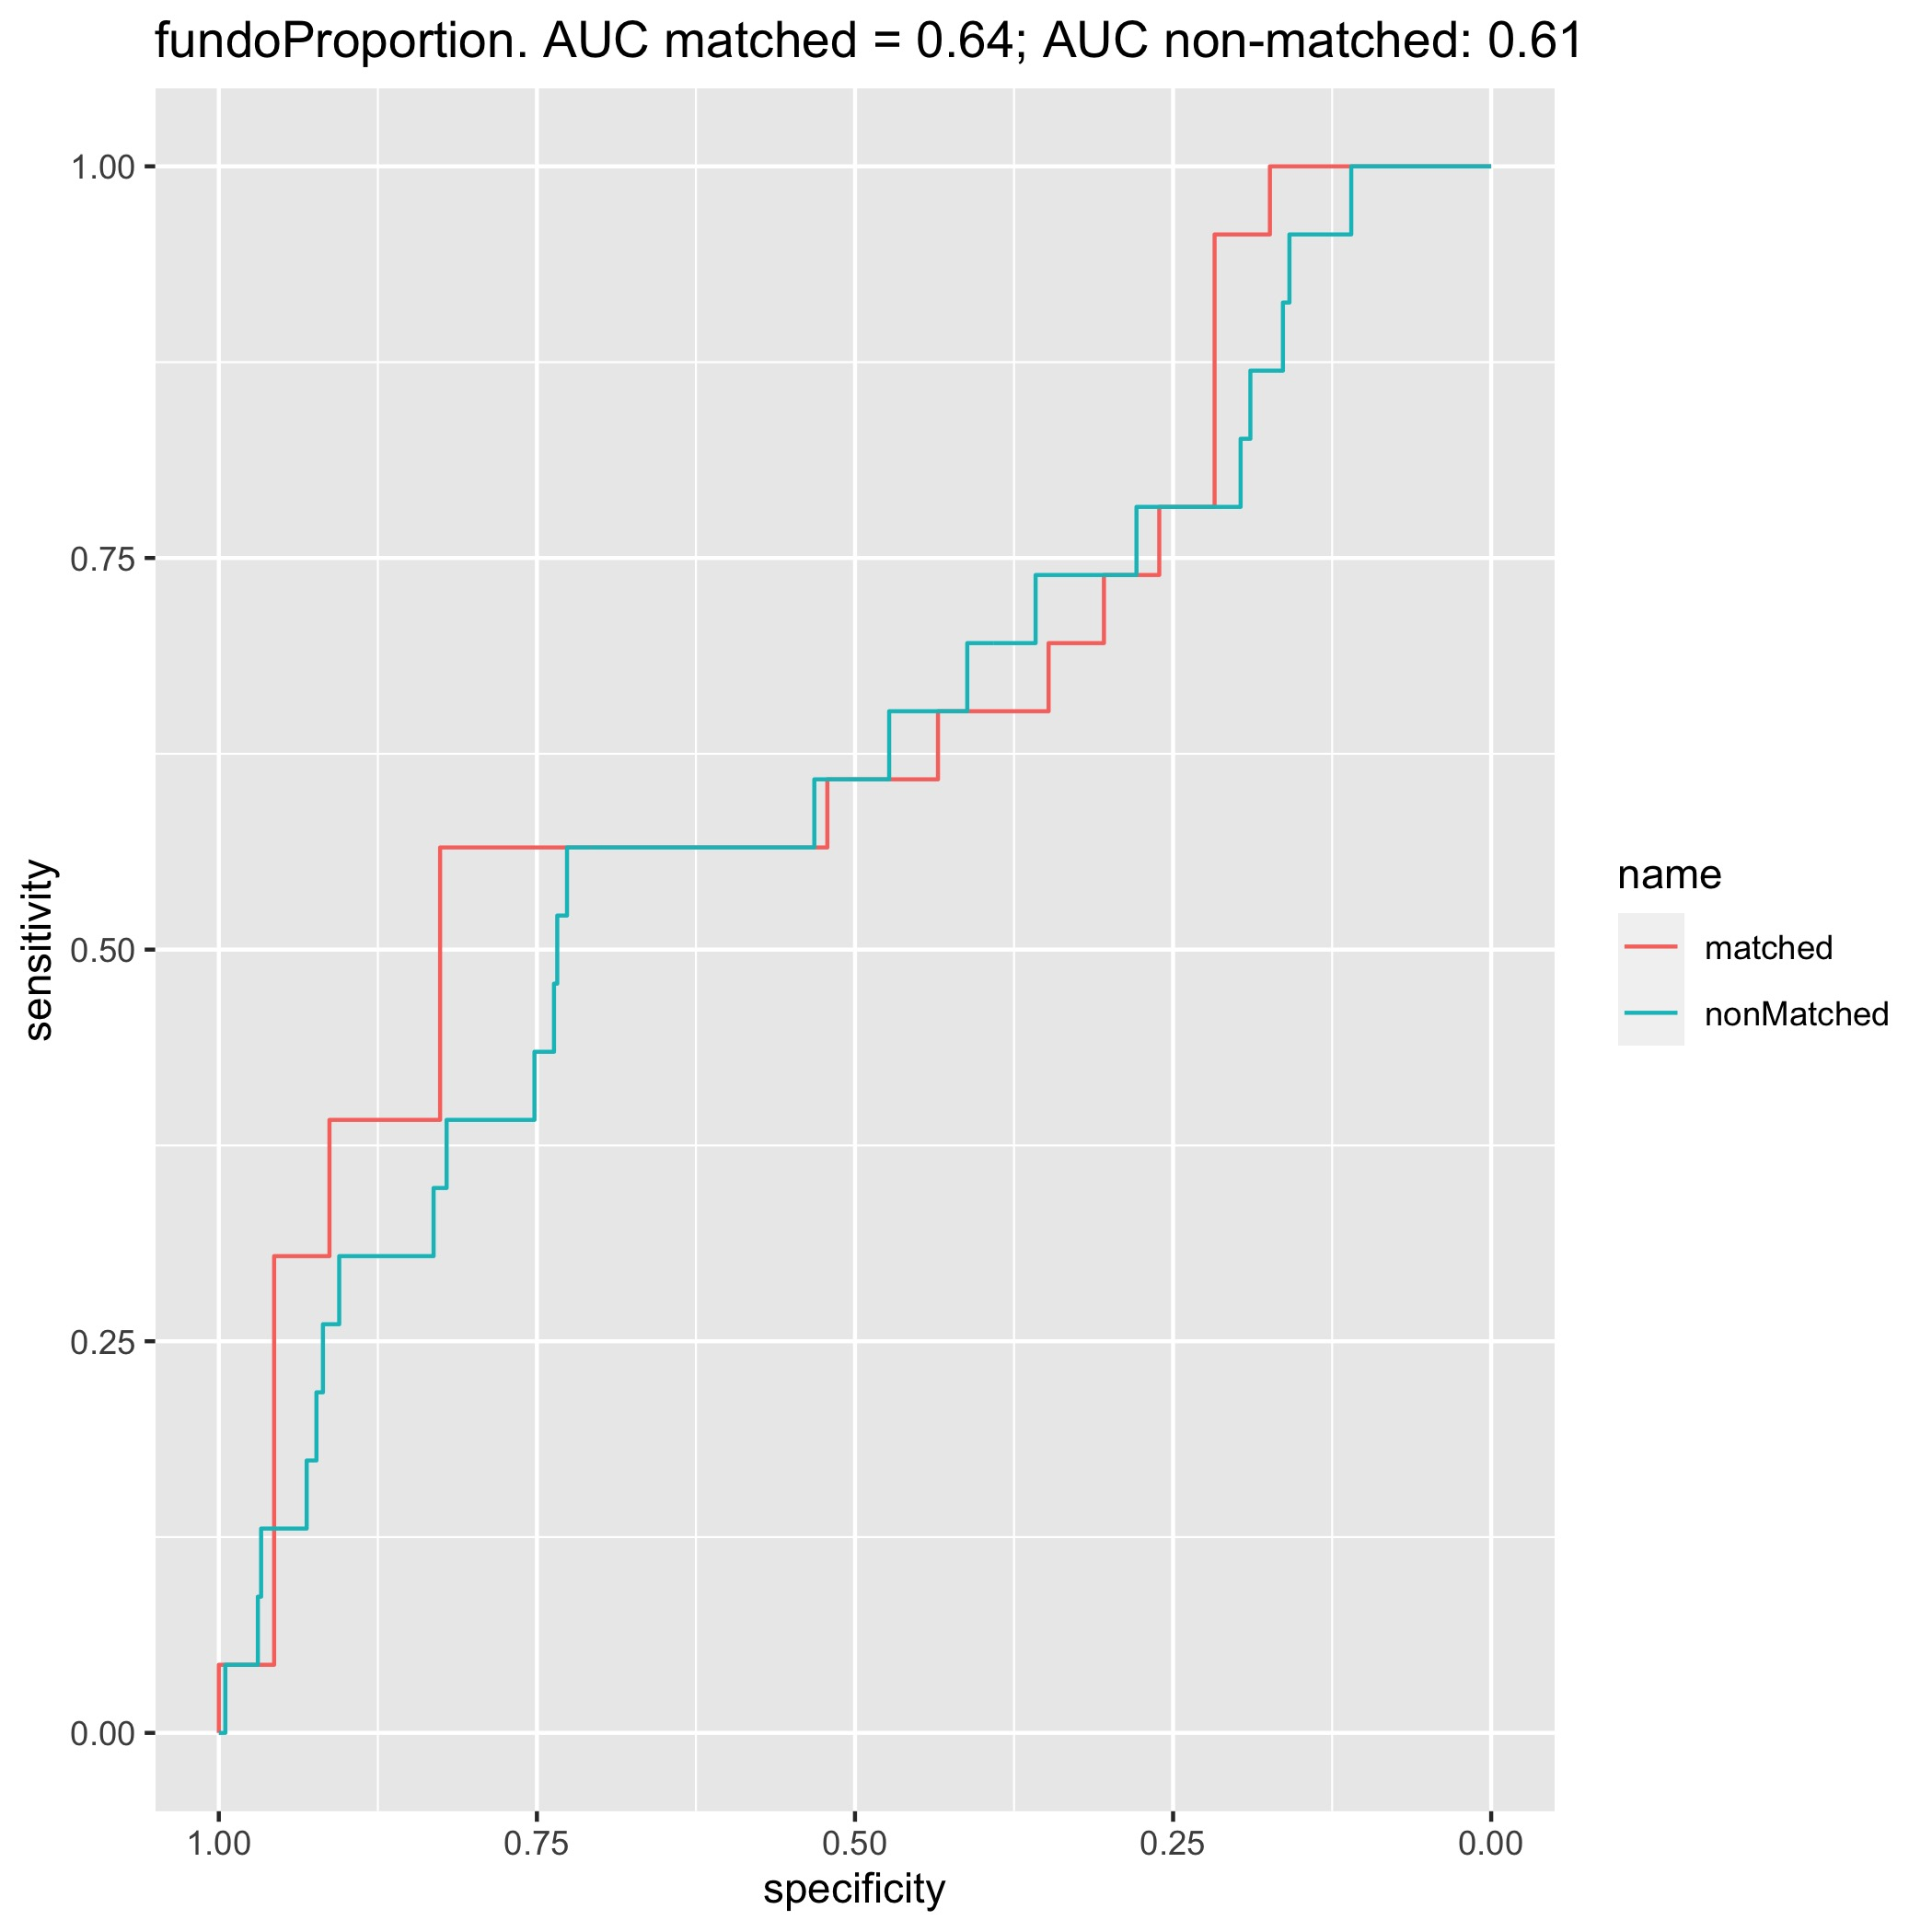
\includegraphics[scale=0.2]{./rocFundoProportion.jpg}}
  \centering
\end{figure}

\begin{figure}[H]
  \caption{ROC curves para targetProportion em samples matched e não matched}
  \noindent\makebox[\textwidth]{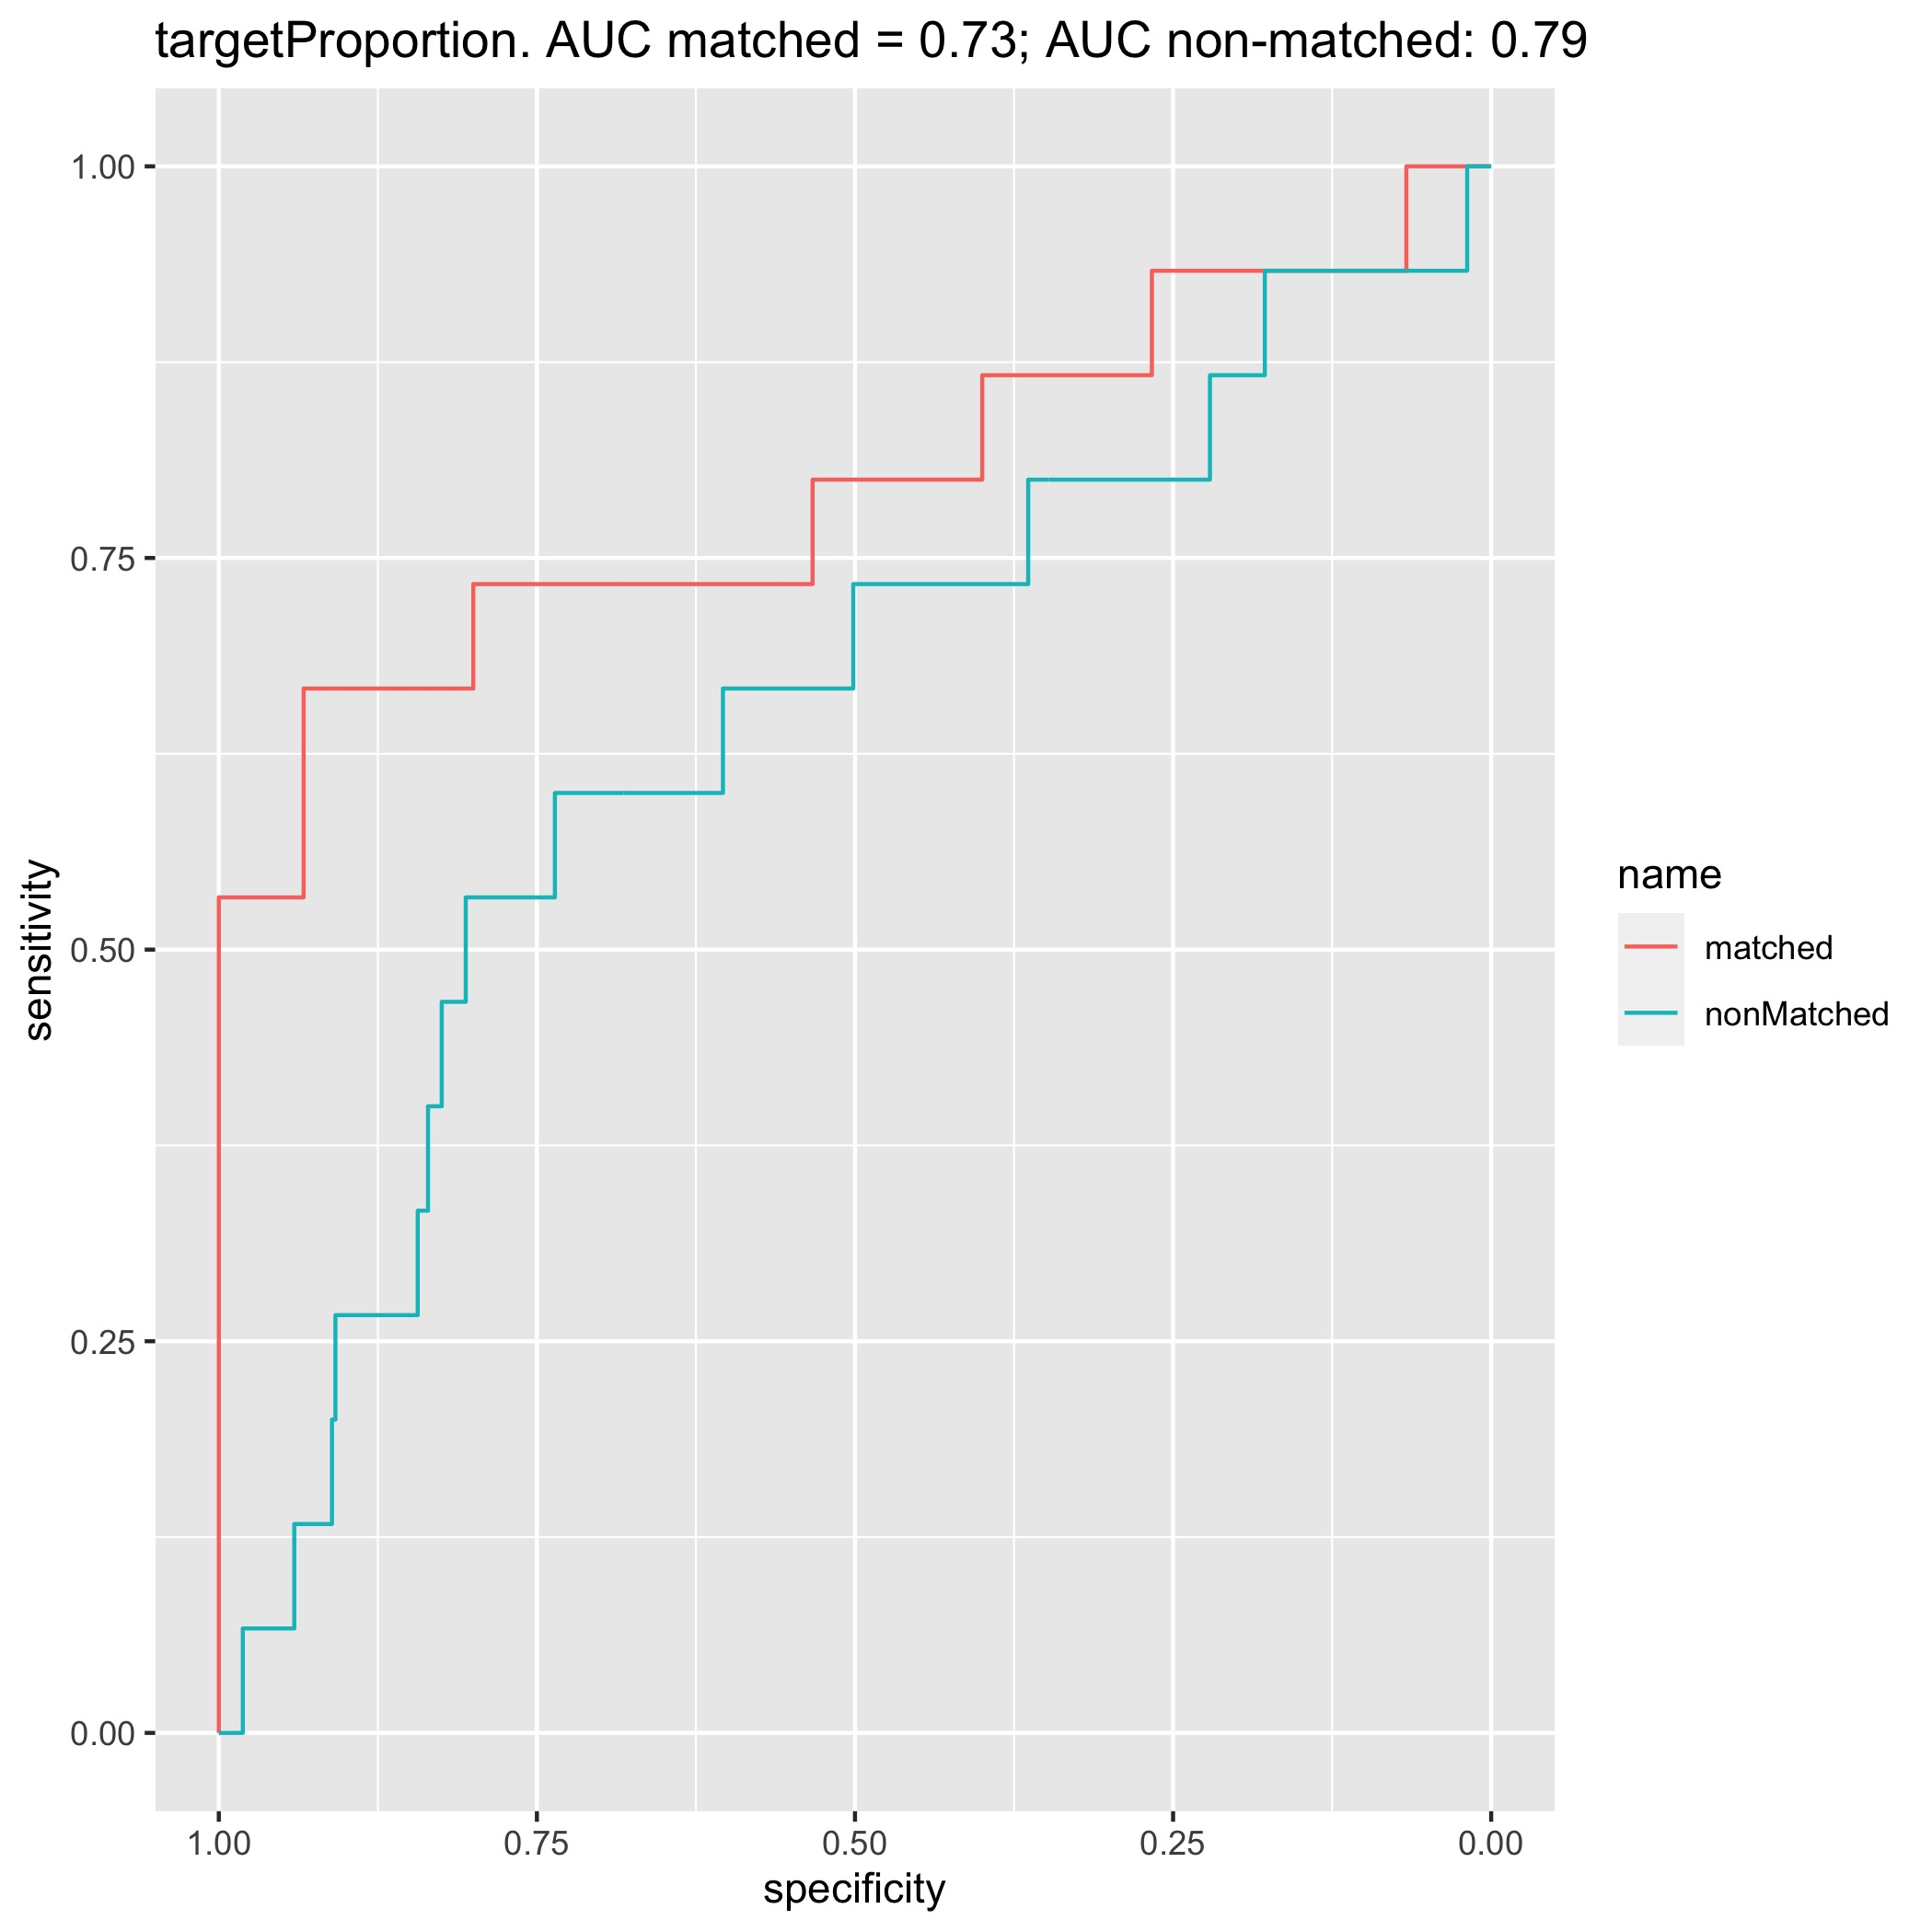
\includegraphics[scale=0.2]{./rocTargetProportion.jpg}}
  \centering
\end{figure}

\subsection{Alternancias}

\begin{figure}[H]
  \caption{Mean number of alternances between two particular AOIs}
  \noindent\makebox[\textwidth]{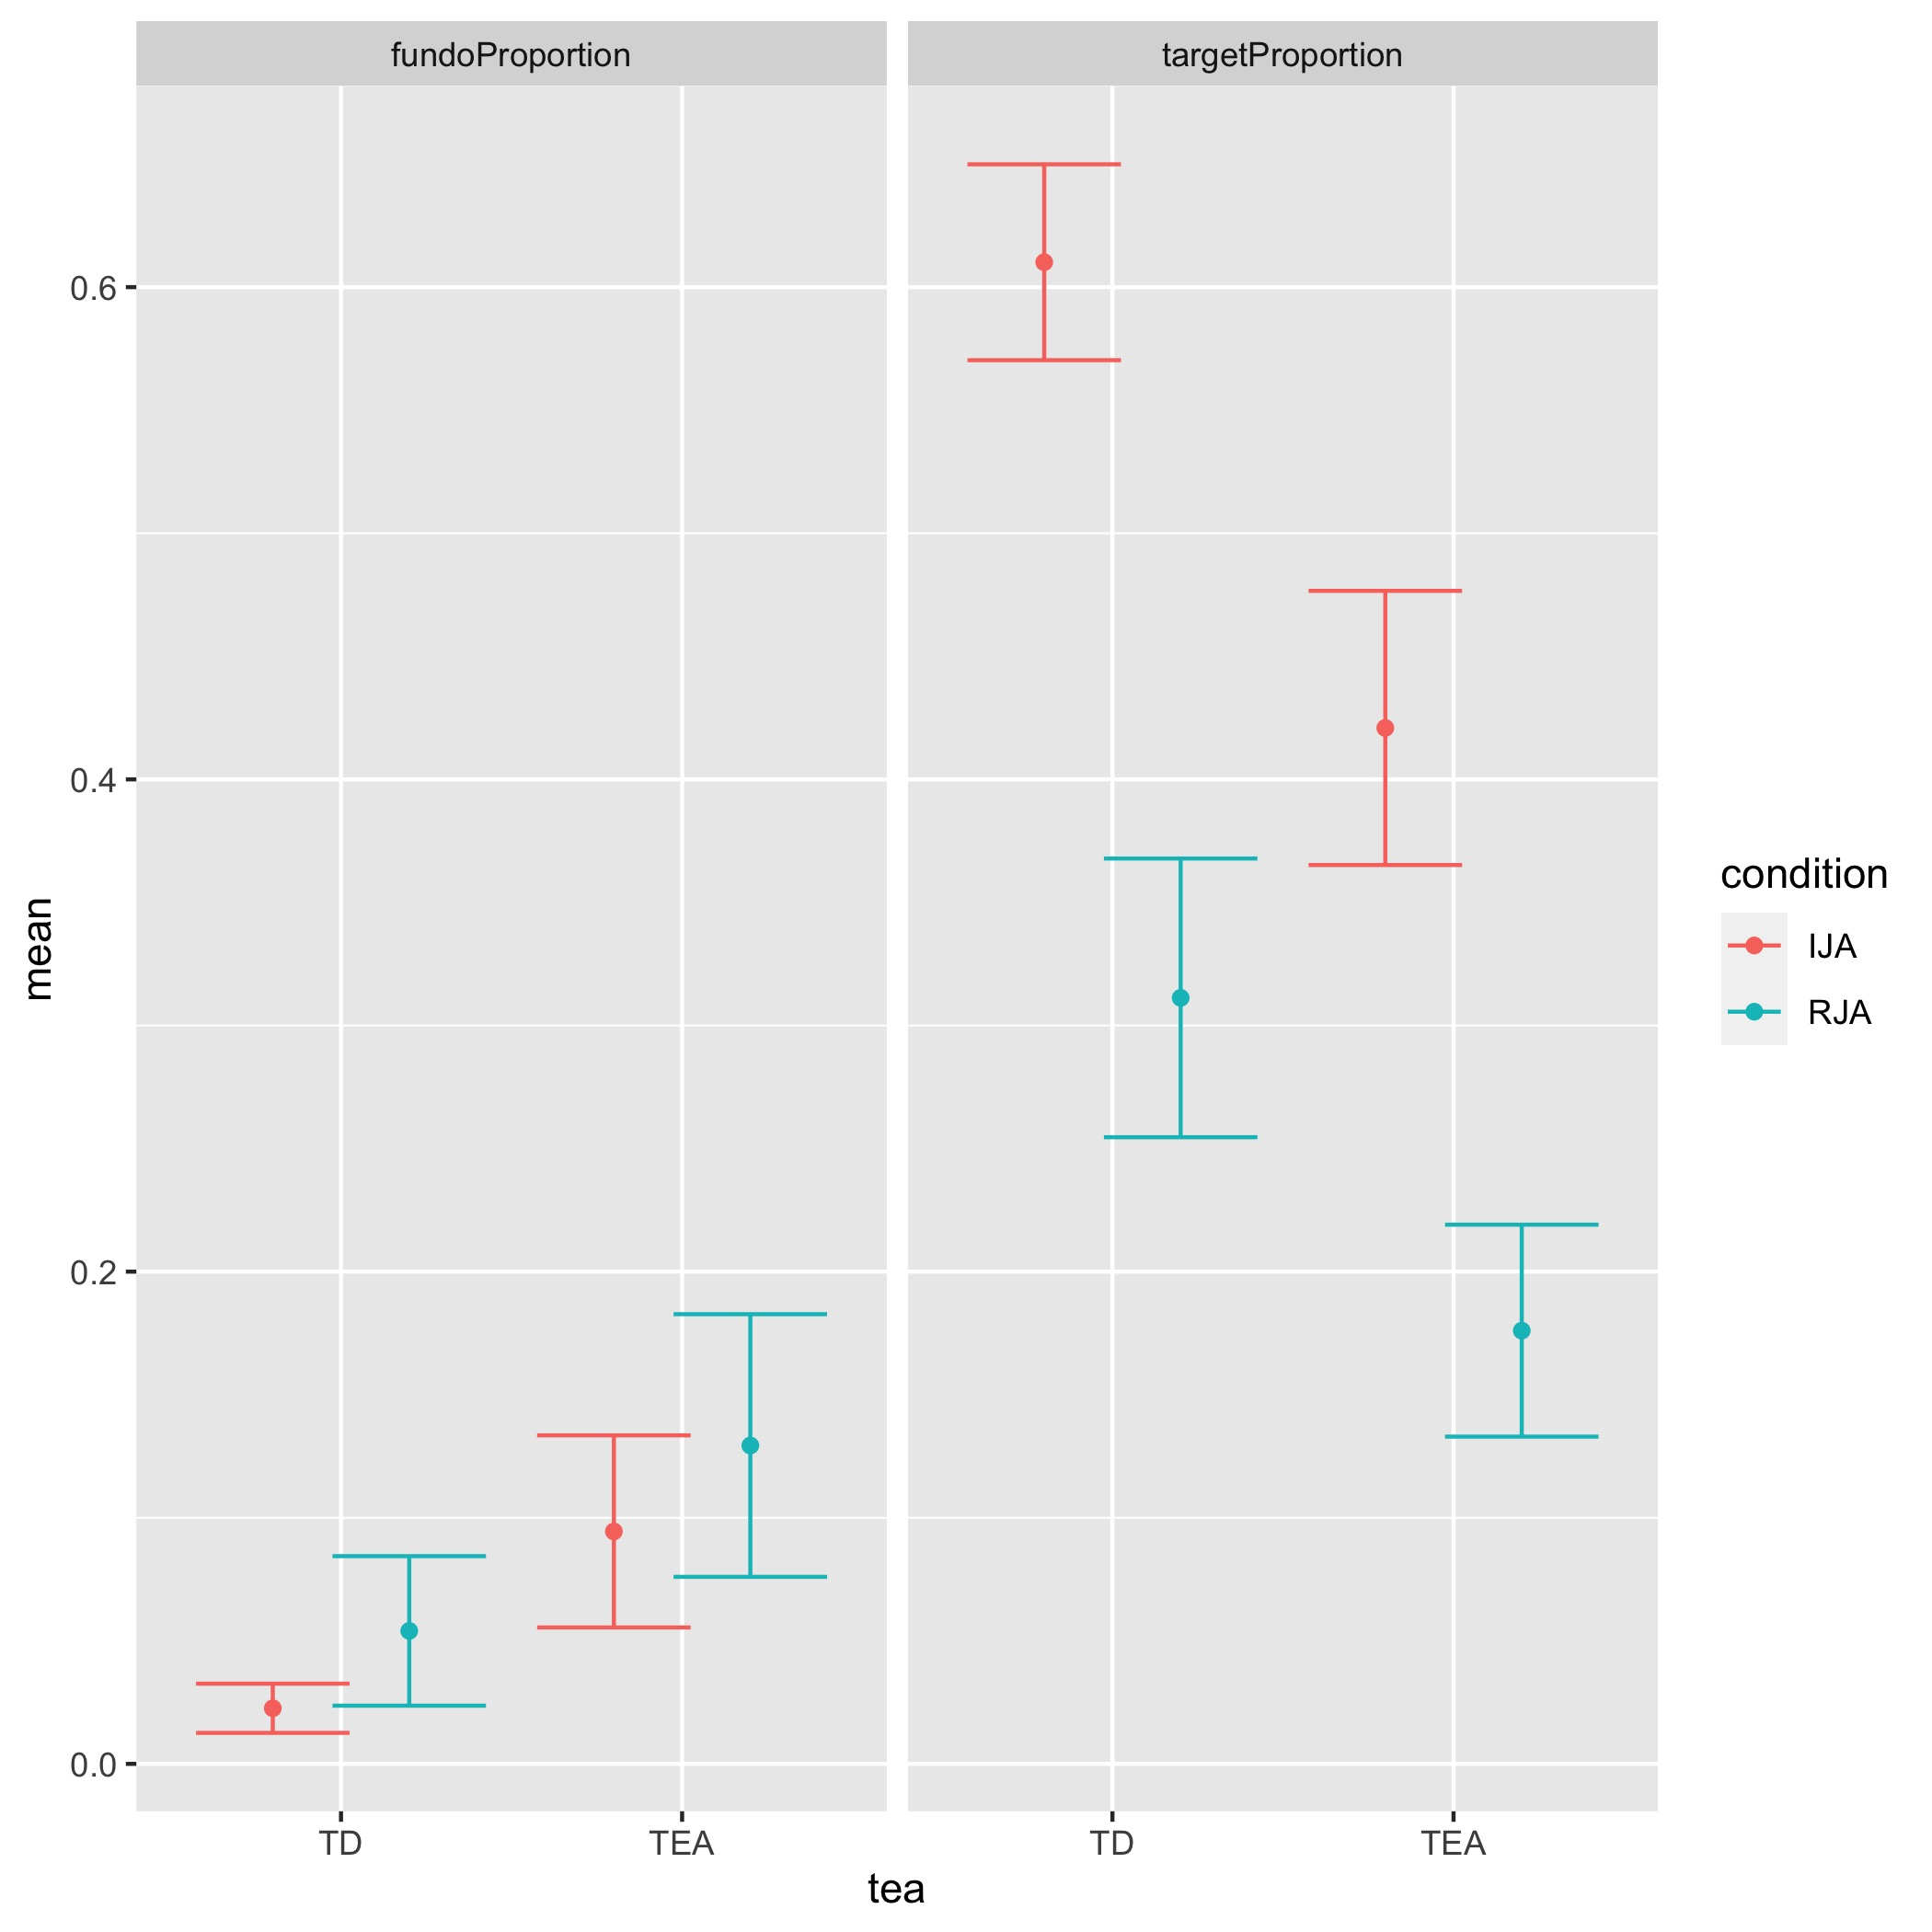
\includegraphics[scale=0.2]{./alternancias.jpg}}
  \centering
\end{figure}

\begin{figure}[H]
  \caption{ROC curves para targetRosto em samples matched e não matched}
  \noindent\makebox[\textwidth]{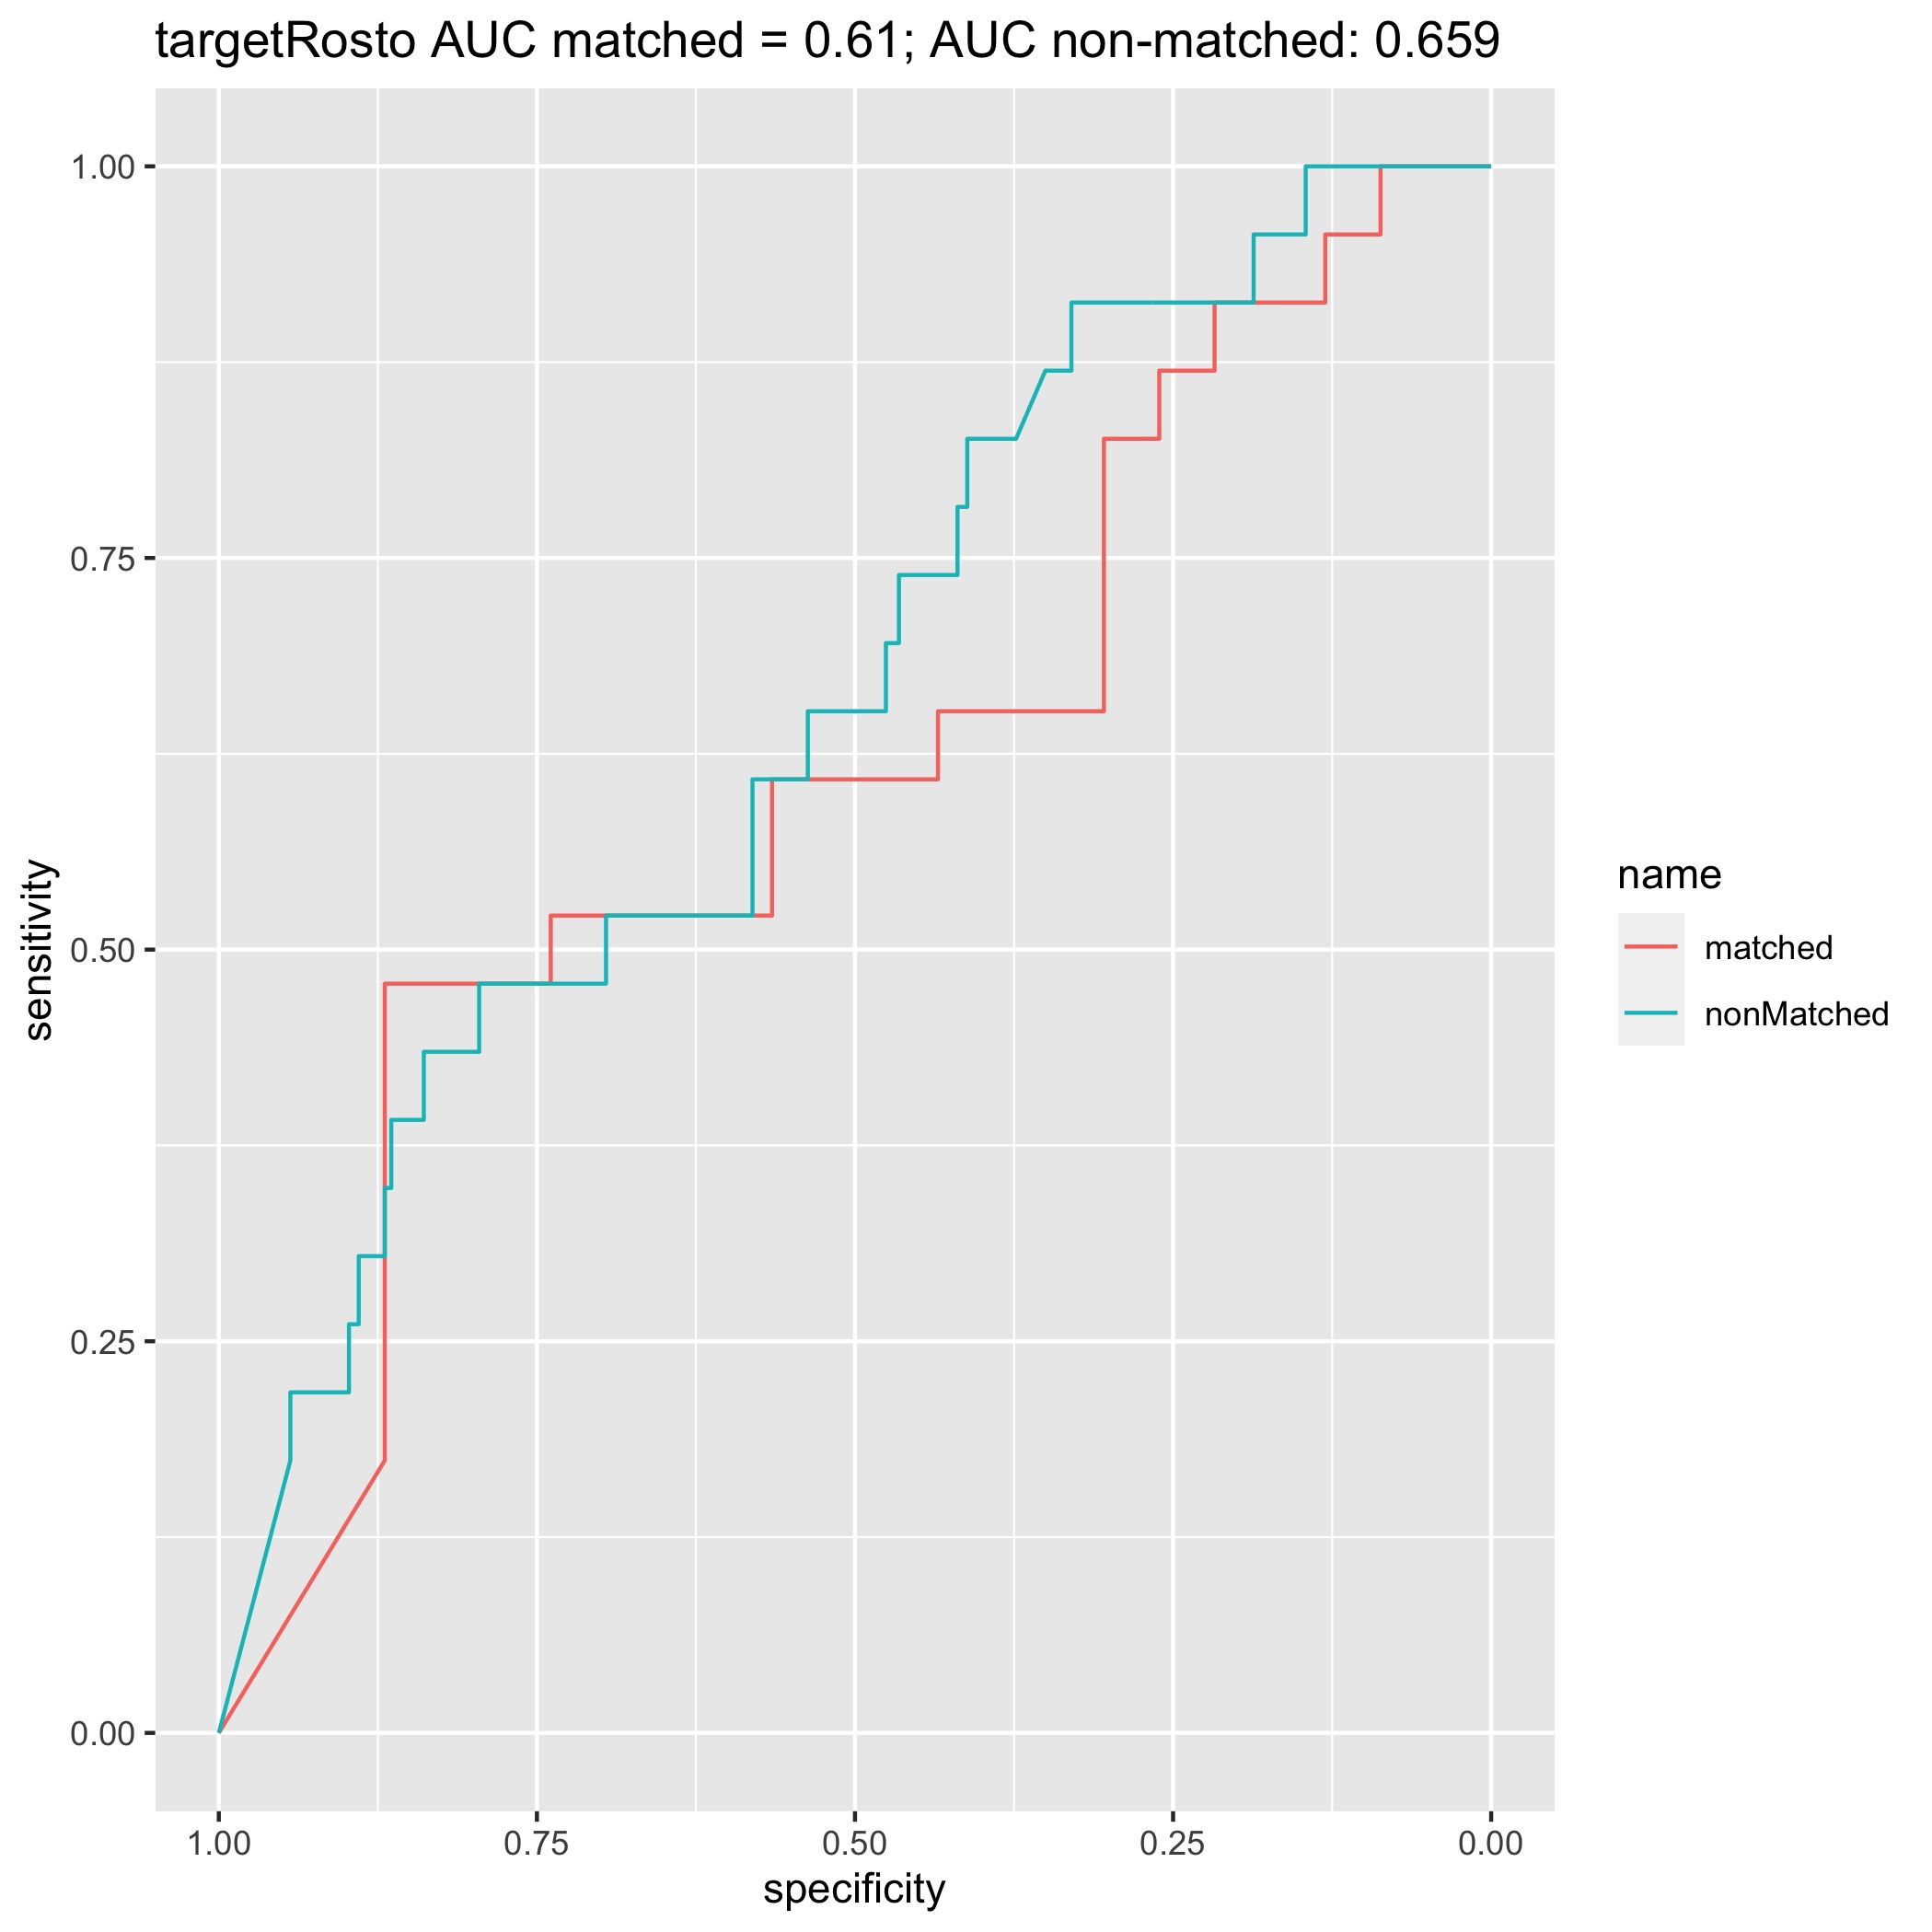
\includegraphics[scale=0.2]{./rocTargetRosto.jpg}}
  \centering
\end{figure}

\begin{figure}[H]
  \caption{ROC curves para rostoTarget em samples matched e não matched}
  \noindent\makebox[\textwidth]{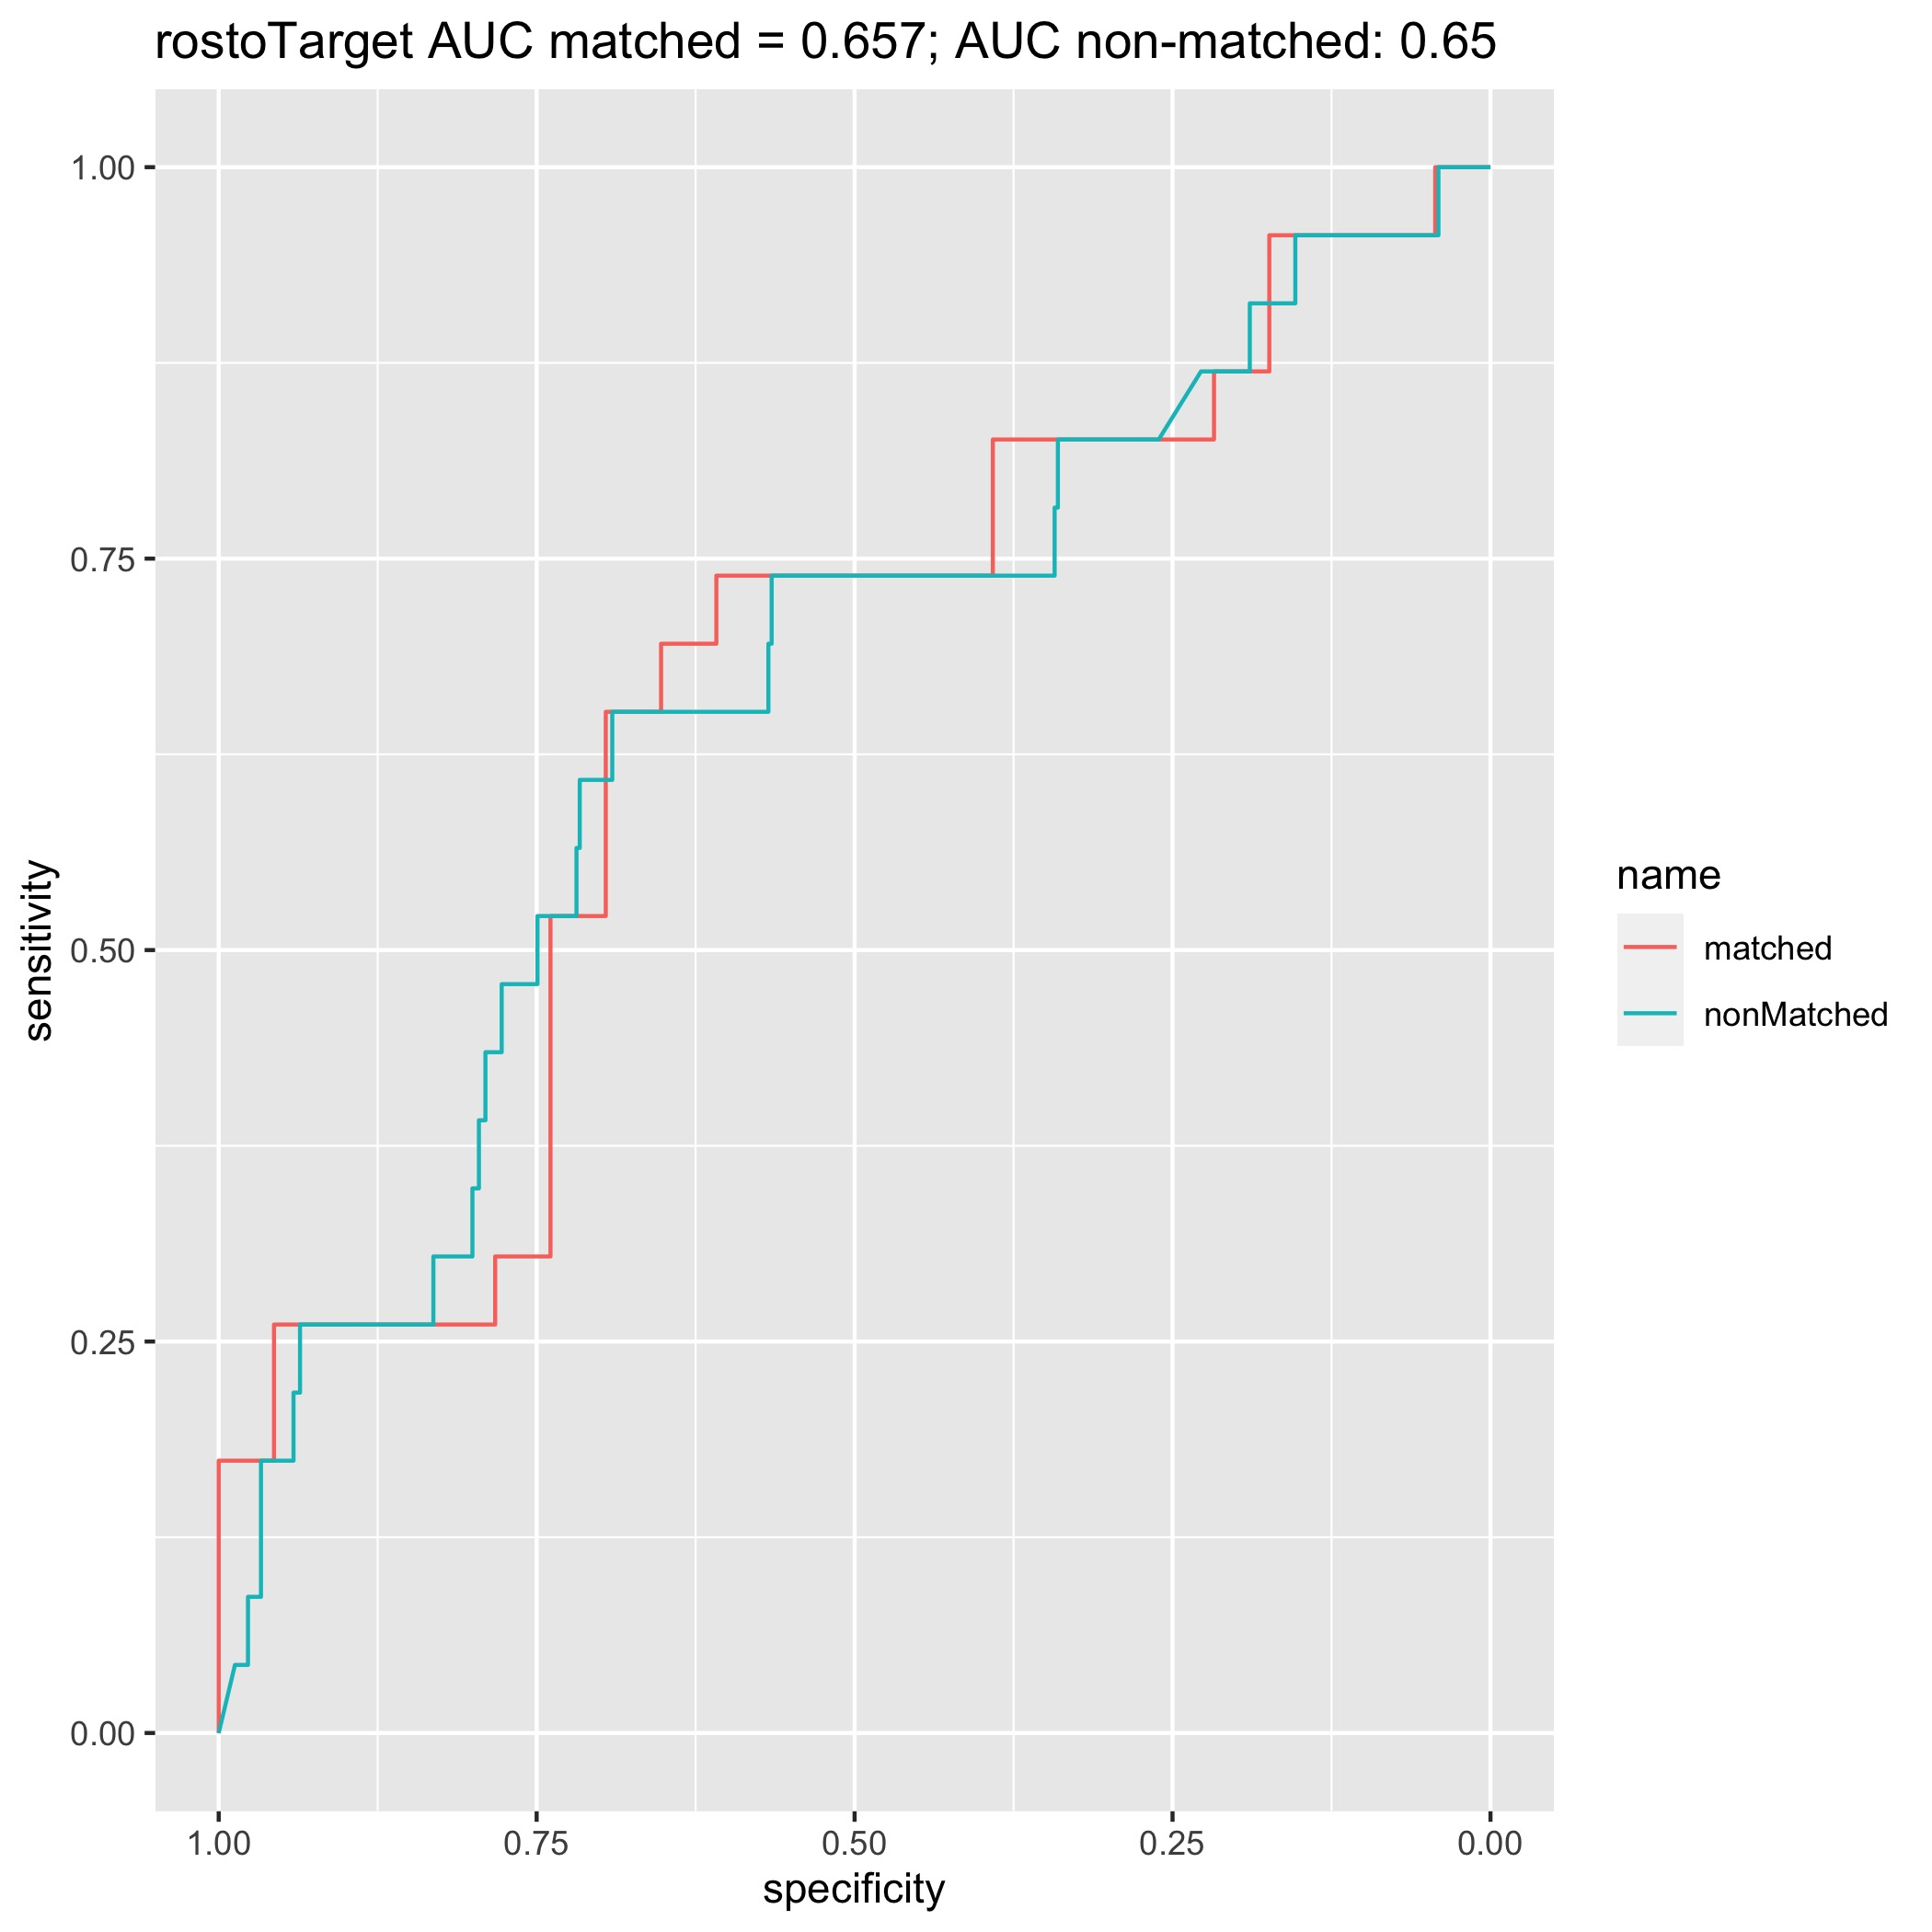
\includegraphics[scale=0.2]{./rocRostoTarget.jpg}}
  \centering
\end{figure}

\end{document}
